\documentclass[usenames,dvipsnames,aspectratio=169]{beamer}
\usepackage[utf8]{inputenc}
\usecolortheme{seahorse}
\usepackage{enumitem,amsmath,xfrac,dsfont,amsfonts,bbm,cancel,euler,ulem}
\usepackage{apacite,natbib}
\usepackage{hyperref}
\usepackage{caption,subcaption,booktabs,multicol,adjustbox}
\usepackage{xcolor}


\title{Innovation, Reallocation, and Growth}
\author{Authors: Daron Acemoglu \and  Ufuk Akcigit \and Harun Alp \\ Nicholas Bloom \and William Kerr \\ \small{Presented by: Jose M. Quintero} }



\AtBeginSection[]
{
  \begin{frame}<beamer>
    \frametitle{Outline}
    \tableofcontents[currentsection]
  \end{frame}
}

\AtBeginSubsection[]
{
   \begin{frame}
        \frametitle{Outline}
        \tableofcontents[currentsubsection]
   \end{frame}
}



\begin{document}

\begin{frame}
  \titlepage
\end{frame}

\begin{frame}{Research Question}
\begin{itemize}[label=\textcolor{teal}{$\blacktriangleright$}]
\vfill
\item Research Question: Industrial policies targeting 
\begin{itemize}[label=\textcolor{teal}{$\star$}]
\item Trade-offs,
\item Reallocation of factors
\item Firm dynamics
\end{itemize}
\vfill
\item Previous literature 
\begin{itemize}[label=\textcolor{teal}{$\star$}]
\item Silent on industrial policy
\item No inefficiency from misallocation.
\end{itemize}
\vfill
\end{itemize}
\end{frame}

\begin{frame}{This paper}
\begin{itemize}[label=\textcolor{teal}{$\blacktriangleright$}]

\vfill
\item Endogenous growth model
\begin{itemize}[label=\textcolor{teal}{$\star$}]
\item Firm heterogeneity
\item Quality obsolescence
\item Multiple exit channels
\end{itemize}
\vfill
\item Match the model to data
\begin{itemize}[label=\textcolor{teal}{$\star$}]
\item LBD (Census data) with USPTO and RAD
\item Firm exit rates
\item Age and size distribution
\item Growth rates
\end{itemize}
\end{itemize}
\end{frame}

\begin{frame}{The Model}

\begin{itemize}[label=\textcolor{teal}{$\blacktriangleright$}]
\vfill
\item Firm dynamics embedded in endogenous growth a la Klette \& Kortum (2004)
\begin{itemize}[label=\textcolor{teal}{$\star$}]
\item Firm level investment decision to grow 
\item Heterogeneity in firm size
\item Competition between incumbents and entrants
\end{itemize}
\pause
\vfill
\item \textcolor{blue}{Firms Exit}
\begin{itemize}[label=\textcolor{teal}{$\star$}]
\item \textit{Creative destruction.}
\item \textcolor{blue}{Endogenous obsolescence}.
\item \textcolor{blue}{Exogenous shock}.
\end{itemize}
\pause
\vfill
\item \textcolor{blue}{Firms Heterogeneity}
\begin{itemize}[label=\textcolor{teal}{$\star$}]
\item \textcolor{blue}{Firm efficiency}: Positive selection.
\item \textcolor{blue}{Type transition}: Negative selection
\end{itemize}
\vfill
\end{itemize}

\end{frame}

\begin{frame}{How do we get some nice results?}
\begin{itemize}[label=\textcolor{teal}{$\blacktriangleright$}]
\item Examining the value function
\begin{align*}
(r+\varphi)V(\mathbf{q}) - \underbrace{\textcolor{blue}{\dot{V}(\mathbf{q})}}_{\frac{\partial V}{\partial q}\textcolor{blue}{\frac{\partial q_j}{\partial w^u}}\frac{\partial w^u}{\partial t}} = \max_{x_f\geq 0 }\begin{cases}
 &\sum_{q_j\in\mathbf{q}}\underbrace{\tilde{\pi}(\textcolor{blue}{q_j})}_{\text{Profits}} - \underbrace{\tilde{w}^s\Phi_j}_{\text{Fix Cost}} - \underbrace{\tilde{w}^s x_f^{\frac{1}{1-\gamma}}}_{\text{R\&D}}  \\
&\sum_{q_j\in\mathbf{q}} \underbrace{\tau\left(V(\mathbf{q}\ominus\{\textcolor{blue}{q_j}\} ) - V(\mathbf{q})\right) }_{\text{Creative Destruction}} \\ 
&\sum_{q_j\in\mathbf{q}} \underbrace{x\left[\mathbb{E}_jV(\mathbf{q}\oplus\{\textcolor{blue}{q_j+\textcolor{blue}{\bar{q}\lambda}} \})-V(\mathbf{q}) \right]}_{\text{Innovation}} 
\end{cases}
\end{align*}
 \item \textcolor{blue}{Blue} terms make the value function separable in $\textcolor{blue}{q_j}$. 

\end{itemize}

\end{frame}

\begin{frame}{It is all reallocation}
\begin{figure}[h]
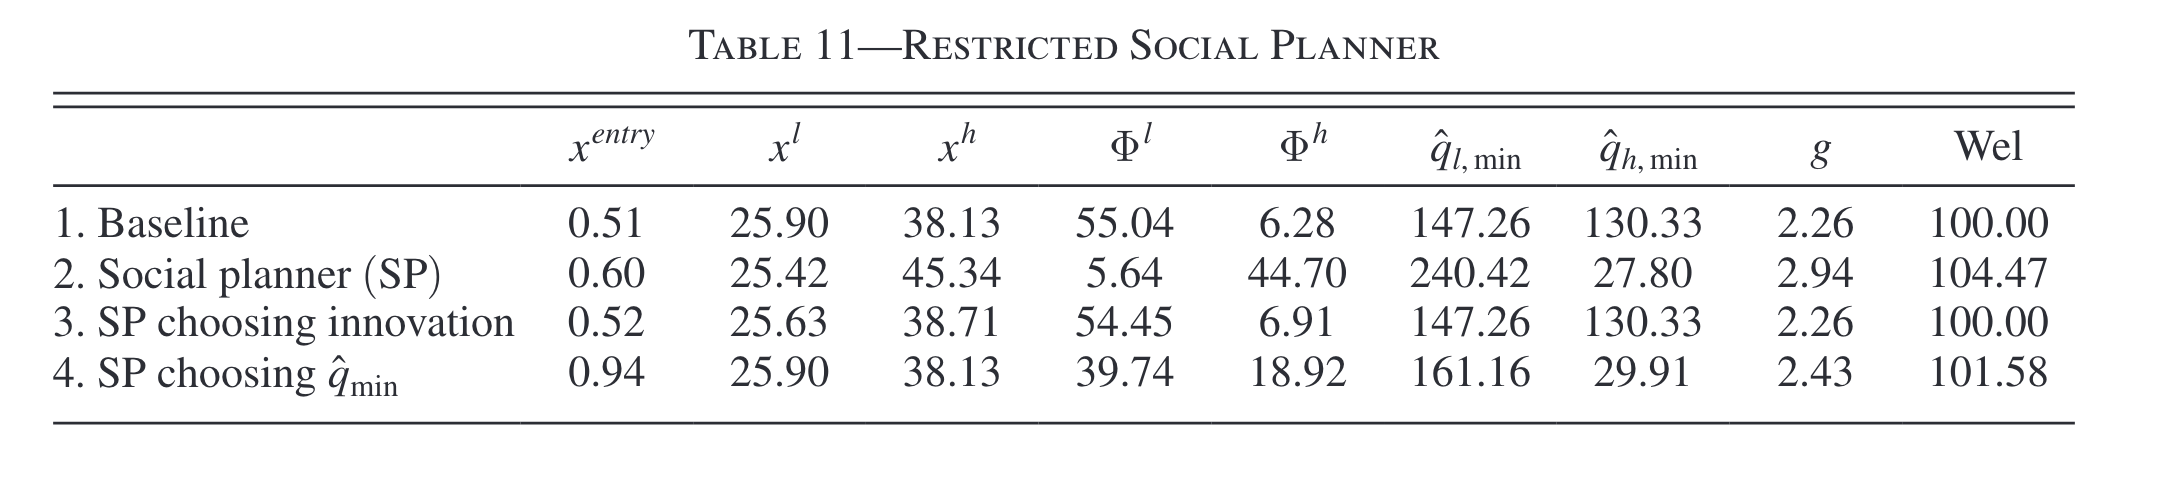
\includegraphics[width=\textwidth]{Figures/week3fig1.png}
\end{figure}
\end{frame}

\begin{frame}{What's next?}

\begin{itemize}[label=\textcolor{teal}{$\blacktriangleright$}]
\vfill
\item Internal innovation  
\begin{itemize}[label=\textcolor{teal}{$\star$}]
\item Every innovation will eventually be lost
\end{itemize}
\vfill
\item Public Finance
\begin{itemize}[label=\textcolor{teal}{$\star$}]
\item Distortionary taxes
\item Mechanism design
\end{itemize}
\vfill 
\item How do expand this framework to explain recent trends?
\begin{itemize}[label=\textcolor{teal}{$\star$}]
\item Market concentration
\item Ownership of the firm: M\&A, VC investment, IPO. 
\end{itemize}
\vfill
\end{itemize}

\end{frame}



\end{document}

